\section{Einführung und Ziele}
\subsection{Aufgabenstellung}
Ausgangspunkt ist die in der Fallstudie \cite{fallstudie2026} beschriebene Analyse-Komponente von \emph{Manufacturing Products}. Mehrere fachlich eigenständige Validierungs- und Simulationsalgorithmen sind dort eng gekoppelt. Lange Laufzeiten einzelner Analysen blockieren dadurch den gesamten Konstruktionsablauf und verschlechtern die Responsiveness der Anwendung.

Der Proof-of-Concept zerlegt diesen Bereich in eigenständig deploybare Microservices. Eine Motorkonfiguration wird persistent verwaltet und anschlie\ss{}end durch mehrere fachlich getrennte Analyse-Services geprüft. Status und Resultate jedes Algorithmus sollen sichtbar sein. Ein einzelner fehlgeschlagener Schritt muss gezielt wiederholt werden können, ohne bereits erfolgreiche Schritte erneut auszuführen.

\subsection{Architekturziele}
\begin{tabularx}{\textwidth}{L{4.3cm}Y}
\toprule
\textbf{Ziel} & \textbf{Konsequenz im Proof-of-Concept} \\
\midrule
Fachliche Zerlegung & Schnitt nach Business Capabilities statt nach technischen Schichten; Strategic DDD mit klaren Bounded Contexts. \\
Lose Kopplung & Kommunikation ausschlie\ss{}lich über explizite REST-Verträge; kein gemeinsam verwendetes Domain-Modul. \\
Ausfallsicherheit & Resilience4j Circuit Breaker kapselt nicht erreichbare Analyse-Services und begrenzt Fehlerkaskaden. \\
Independent Deployability & Jeder Microservice besitzt einen eigenen Build und läuft in einem eigenen Docker-Container. \\
Monitorability & Status, Einzelresultate und Gesamtergebnis sind über eine Analyse-ID nachvollziehbar. \\
Responsiveness & Der Start einer Analyse blockiert nicht bis zum Ende aller Algorithmen. \\
Testbarkeit & Happy Path, Fehlerfall und Retry sind automatisiert sowie über die API reproduzierbar. \\
\bottomrule
\end{tabularx}

\subsection{Wesentliche fachliche Anforderungen}
\begin{itemize}
  \item Engine-Konfiguration erfassen, validieren, speichern und laden.
  \item Qualitätsanalyse für eine bestehende Konfiguration starten.
  \item Mindestens vier fachlich getrennte Analysealgorithmen als eigenständige Microservices verwenden.
  \item Status \code{PENDING}, \code{RUNNING}, \code{READY} und \code{FAILED} pro Algorithmus verwalten.
  \item Einzelresultate sowie ein \emph{Overall Result} bereitstellen.
  \item Fehlgeschlagene Algorithmen einzeln wiederholen können.
  \item Ausfälle einzelner Analyse-Services kontrolliert behandeln.
  \item Den PoC mit Docker und Docker Compose betreiben.
\end{itemize}

\newpage

\section{Randbedingungen}
\begin{tabularx}{\textwidth}{L{4.2cm}Y}
\toprule
\textbf{Technologie} & \textbf{Verwendung} \\
\midrule
Java 21 / Spring Boot & Implementierung der sechs Microservices und REST-Schnittstellen. \\
React / Vite / MUI & Web-Oberfläche für Konfiguration, Statusübersicht, Retry und Overall Result. \\
H2 / Spring Data JPA & Persistenz in Configuration Management und Analysis Management. \\
Resilience4j & Umsetzung des Circuit-Breaker-Patterns für Service-zu-Service-Aufrufe. \\
Docker / Docker Compose & Isolierte Bereitstellung und lokale Komposition aller Services. \\
JUnit 5 / Mockito / Postman & Automatisierte Tests sowie manuelle Demonstration der API. \\
PlantUML / TikZ & Architekturdiagramme und Dokumentation. \\
\bottomrule
\end{tabularx}

Nicht Bestandteil dieses Proof-of-Concepts sind eine reale physikalische Motorsimulation, die vollständige Migration der bestehenden Unternehmenssoftware, Kubernetes oder Cloud-Deployment sowie eine Camunda- oder MCP-Orchestration des Order-Fulfillment-Prozesses. Kafka wird im Kernumfang nicht verwendet.

Die vier Analyse-Services arbeiten daher mit vereinfachten, deterministischen Prüfregeln. Im Mittelpunkt stehen die Architekturentscheidungen, Servicegrenzen, Datenhoheit, Resilience und Nachvollziehbarkeit der Verarbeitung.

\section{Kontextabgrenzung}
Der primäre Akteur ist der \textbf{Ingenieur}. Im Prüfungsszenario übernimmt diese Rolle der Demo-Operator. Er erstellt oder lädt eine Motorkonfiguration, startet die Qualitätsanalyse, beobachtet den Bearbeitungsstatus und stö\ss{}t bei Bedarf einen Retry an.

\begin{figure}[h]
  \centering
  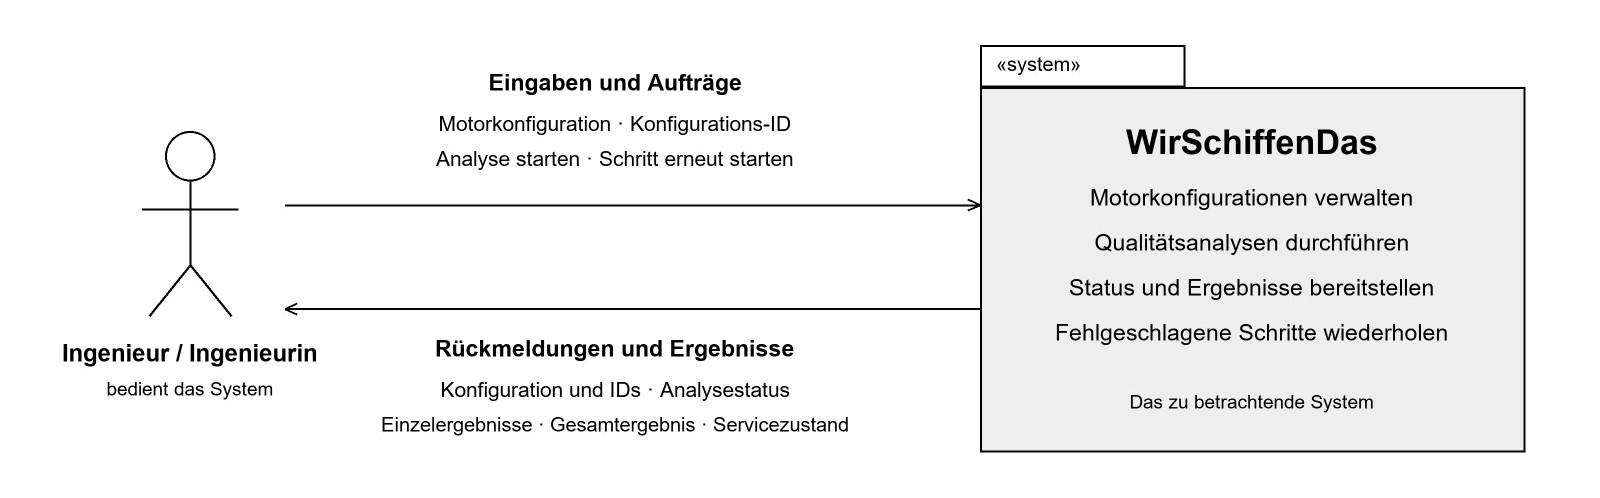
\includegraphics[width=\textwidth]{../diagrams/Kontextsicht.jpeg}
  \caption{Kontextsicht: Akteur, Frontend und Engine Quality Analysis.}
\end{figure}

Die Systemgrenze umfasst ausschlie\ss{}lich den PoC der Engine Quality Analysis. Externe Unternehmenssysteme und der vollständige Order-Fulfillment-Prozess liegen au\ss{}erhalb dieser Dokumentation.
